% CHAPTER 2

\chapter{Design of a digital ARTVA \label{ch:chapter2}}
\minitoc
%% Enlarge array size
\renewcommand{\arraystretch}{2}

In this chapter we will try to design a digital receiver for the ARTVA signal. Before starting with the design, \emph{ARTVA signal} is analyzed in detail, with the derivation of a simplified model of field pattern that could be used  for the implementation of the searching algorithm. After, ferrite antennas are analyzed, as they are the only way to receive such a long wavelength. In the last part of the chapter the circuitry for the ARTVA receiver is shown.

\section{Analysis of transmitting pattern}

A formal model of the transmitting pattern is fundamental for the implementation of the searching algorithm. We start from the basic Maxwell equation and we arrive to a simpler model numerically usable.

As we will see, radiating pattern is quite complex due to the fact that we are working in the \textbf{near--field} region, condition that constraint not to use classical DoA\marginnote{\emph{DoA}: Direction of Arrival}, such as MUSIC or ESPRIT, that operates in far-field condition and at higher frequencies. DoA systems for long waves usually requires too big electro--mechanical devices.

\subsection{Maxwell's Equations}
The following investigation is based upon Maxwell's Equation, in which the magnetic permeability $\magperm$ and $\dielettrico$ is considered as a constant (the radiation is assumed to propagate at speed of light in air). Also we consider some field properties, that are function of radio distance and time:
\[
f(\radiodist,t) = f \qquad f \in \left[\; \chargedens,\; \currdens,\; \efield,\; \bfield,\; \hfield \; \right]
\]
The equations that rule the induction are the \emph{Gauss equation of magnetic induction} and the \emph{Faraday law of electric induction}:
\begin{equation}
\nabla\cdot\bfield = 0
\label{eq:gauss1}
\end{equation}
\begin{equation}
\nabla\times\efield = -\partialt \bfield
\label{eq:faraday}
\end{equation}
while the equations that rule the interaction with material are \emph{Gauss equation} and \emph{Ampere law}:
\begin{equation}
\nabla\cdot\efield = \dfrac{\chargedens}{{\dielettrico}_0}
\label{eq:gauss2}
\end{equation}
\begin{equation}
\nabla\times\bfield = {\magperm}_0 \left( \currdens + {\dielettrico}_0 \partialt \efield \right)
\label{eq:ampere}
\end{equation}

\subsection{EM field dynamic potentials}

Starting from equation \ref{eq:gauss1}, we can define a vectorial function called \emph{potential vector} $\afield$ of $\bfield$:
\begin{equation}
\bfield = \nabla\times\afield
\label{eq:potvett}
\end{equation}
\marginnote{The existence od $\afield$ is verified by property of $\nabla$ operator, whom states that the divergence of a curl of a vector field is zero} Putting \ref{eq:potvett} in \ref{eq:faraday}:
\[
\nabla\times\efield = - \partialt \left( \nabla\times\afield \right)
\]
\begin{equation}
\nabla\times\left( \efield + \partialtarg{\afield} \right) = 0
\end{equation}
From the previous equation it is evident that the argument between parenthesis is in reality an irrotational vector field, thus a potential function exists such that:
\[
-\nabla\scpot = \efield + \partialtarg{\afield}
\]
and we derive the following definition of electric field:
\begin{equation}
\efield = - \nabla \scpot - \partialtarg{\afield}
\label{eq:efieldvett}
\end{equation}
Equation \ref{eq:potvett} and \ref{eq:efieldvett} are used to express a new formulation for the Maxwell's equation based upon vector potential\sidenote{The proof is in chapter appendix \ref{eq:evidence1}}:
\begin{equation}
\begin{array}{rcl}
\nabla^2\scpot + \partialt \nabla \cdot \afield & = & - \dfrac{\chargedens}{\dielettrico_0} \\
\nabla^2 \afield - \dfrac{1}{\velocitaluce^2} \partialttarg{\afield} - \nabla\left( \nabla \cdot \afield + \dfrac{1}{\velocitaluce^2} \partialtarg{\scpot} \right) & = & -\magperm_0 \currdens
\end{array}
\label{eq:potvecmaxwell}
\end{equation}
Those equation, even if the evident complexity, could be resolved as a well posed boundaries condition problem. Equation are coupled with the current formulation, but could be decoupled using the \textbf{Gauge transformation}, also called \textbf{recalibration map}, that are in the form:
\begin{equation}
\left\{ \begin{array}{rcl}
\afield' & \mapsto & \afield + \nabla \lorentz \\
\scpot' & \mapsto & \scpot - \partialtarg{\lorentz}
\end{array}
\right.
\end{equation}
in which $\lorentz = \lorentz(\radiodist,t) \in C^2$. As proofed in \ref{eq:prooftransformationmap}, this map represents an invariance for dynamic potential formulation. If we consider a $\lorentz$ such that verifies the \textbf{Lorentz equation}
\begin{equation}
\nabla \cdot \afield' = - \dfrac{1}{\velocitaluce^2} \partialtarg{\scpot'}
\end{equation}
we obtain in the previous equations the decoupled version:
\begin{equation}
\begin{array}{rcl}
\nabla^2 \scpot - \dfrac{1}{\velocitaluce^2} \partialttarg{\scpot} & = & - \dfrac{\chargedens}{\dielettrico_0} \\
\nabla^2 \afield - \dfrac{1}{\velocitaluce^2} \partialttarg{\afield} & = & - \magperm_0 \currdens 
\end{array}
\end{equation}
Those dynamic equations describe the time evolution of an EM--field. If field sources are localized in a finite region, those equations admit as solution a generalization of the well know solution of stationary case, called retarded potential:
\begin{equation}
\begin{array}{rcl}
\scpot(\radiodist,t) & = & \dfrac{1}{4\pi \dielettrico_0} \displaystyle\iiint\limits_{\Omega} \dfrac{1}{\mid \radiodist - \radiodist' \mid} \chargedens\left( \radiodist',t-\dfrac{\mid \radiodist - \radiodist' \mid}{\velocitaluce} \right) d\radiodist   \\
\afield(\radiodist,t) & = & \dfrac{\magperm_0}{4\pi} \displaystyle\iiint\limits_{\Omega} \dfrac{1}{\mid \radiodist - \radiodist' \mid} \currdens\left( \radiodist',t-\dfrac{\mid \radiodist - \radiodist' \mid}{\velocitaluce} \right) d\radiodist 
\end{array}
\end{equation}
in which the vector distance $\radiodist - \radiodist'$ is the distance between the point where retarded potential is evaluated and the point where the element of volume $d\radiodist$ of the localized sources is located. The delay is inserted by the definition of time:
\[
t_r = t - \dfrac{\mid \radiodist - \radiodist' \mid}{c}
\]

\subsection{Magnetic dipole radiation}

\begin{figure}[h]
	\centering
	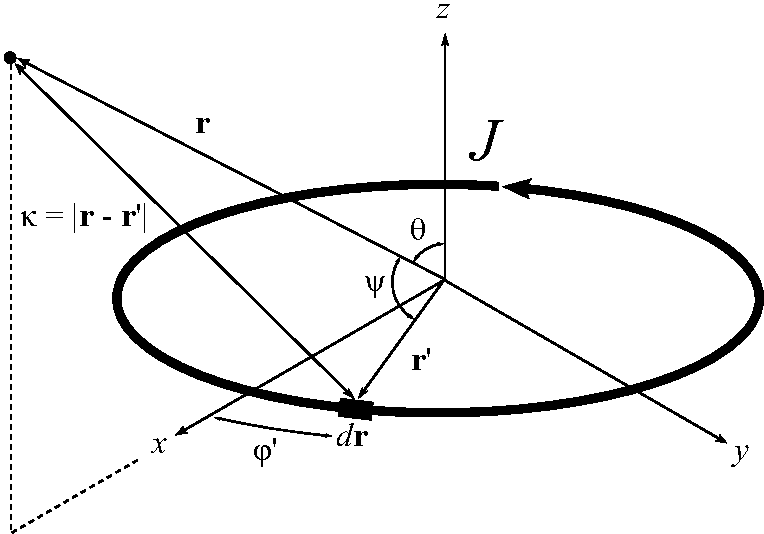
\includegraphics[width=8cm]{ch2/img/dipolo_magnetico.pdf}
	\caption{Formulation of a magnetic dipole problem}
	\label{eq:dipolomagnetico}
	\forceversofloat
\end{figure}
Our antenna may be seen as an ideal magnetic dipole. The transmitting antenna is a solenoid around with a ferrite core, that acts as source of the electro--magnetic field. The source is subject to a dipole magnetic moment induced by the current $J = J_0 \cos(\omegaarva t)$, with no free charges (null scalar potential). The magnetic dipole moment is:
\begin{equation}
\magdipole = \pi r'^2\; J \vrz = m_0 \cos(\omegaarva t) \vrz
\end{equation}
From figure \ref{eq:dipolomagnetico} we define the retarded potential equation, with $\kappa = \mid \radiodist-\radiodist'\mid$:
\[
\afield(\radiodist,t) = \dfrac{\magperm_0}{4\pi}\int{\dfrac{J_0\cos(\omegaarva (t - \kappa/c))}{r}}
\]
In the hypothesis of $\radiodist\parallel\vrz\times\vrx$, we obtain a vector $\afield$ directed along $\vry$:
\[\begin{array}{rcl}
\radiodist & = & r \sin(\theta) \vrx + r \cos(\theta) \vrz \\
\radiodist' & = & r' \cos(\varphi') \vrx + r' \sin(\varphi') \vry \\
\kappa & = & \sqrt{(\radiodist - \radiodist')\cdot(\radiodist - \radiodist')}
\end{array}\]
Those elements in retarded potential formulation lead us to the integral formulation that has only one angular dependency:
\begin{equation}
\label{eq:integraledacalc}
\afield(\radiodist,t) = \dfrac{\magperm_0 J_0 r'}{4\pi}\int\limits_{0}^{2\pi}{\dfrac{\cos(\omegaarva (t - \kappa/c))}{\kappa} \cos(\varphi') d\varphi' \hat{\phi}}
\end{equation}
The solution of this integral is reported in appendix; we recall only on the simplification used:
\begin{itemize}
\item we assume $r' \ll r$
\item we assume $r' \ll \lambda = 2\pi c/\omegaarva$
\end{itemize}
that brings us to the following solution:
\begin{equation}
\label{eq:soluzioneint}
\afield(\radiodist,t) = \dfrac{\magperm_0 m_0}{4\pi r}\,\sin(\theta)\left( \dfrac{1}{r} \sin\left(\omegaarva(t-r/c)\right) - \dfrac{\omegaarva}{r}\cos\left(\omegaarva(t-r/c)\right)\right)\hat{\phi}
\end{equation}
in which $m_0$ identifies the total dipole moment, considering also the number of the coils of antenna. The rest of the equation describes the propagation of the transmission in near--field conditions. With null scalar potential we obtain the electric field and the magnetic field from the equations:
\marginnote{In polar coordinates: \newline $\nabla=\left[ \begin{array}{c} \dfrac{\partial}{\partial r} \\ \dfrac{1}{r}\;\dfrac{\partial}{\partial\theta} \\ \dfrac{1}{r \sin(\theta)}\;\dfrac{\partial}{\partial\phi} \end{array} \right]$}
\begin{equation}
\begin{array}{rcl}
\efield & = & - \partialtarg{\afield} \\
\bfield & = & \nabla\times\afield 
\end{array}
\end{equation}
The application of differential operator $\nabla$:
\begin{equation}
\efield = \left[ \begin{array}{c} 0 \\ 0 \\ \partialtarg{A_{\phi}} \end{array} \right]
\end{equation}
\begin{equation}
\bfield = \left[ \begin{array}{c} \dfrac{1}{r}\;\dfrac{\partial A_{\phi}}{\partial \theta} \\ - \dfrac{\partial A_{\phi}}{\partial r} \\ 0 \end{array} \right]
\end{equation}
The final formulation of the EM field is:
\begin{equation}
\begin{array}{rcl}
\label{eq:campidef1}
\tau & = &  t - \dfrac{r}{\velocitaluce} \\
E_{\phi} & = & \dfrac{\magperm_0 m_0}{4\pi}\sin(\theta)\left( \dfrac{\omegaarva}{r^2}\sin\left( \omegaarva\tau \right) + \dfrac{\omegaarva^2}{c}\cos\left( \omegaarva\tau \right) \right) \\
B_{r} & = & \dfrac{\magperm_0 m_0}{2\pi r^2}\cos(\theta)\left( \dfrac{1}{r}\cos\left( \omegaarva\tau \right) + \dfrac{\omegaarva}{c}\sin\left( \omegaarva\tau \right) \right) \\
B_{\theta} & = & \dfrac{\magperm_0 m_0}{4 \pi r^3 c^2}\sin(\theta)\left( \left( \velocitaluce^2 - \omegaarva^2 r^2 \right)\cos\left( \omegaarva\tau \right) + \omegaarva r \velocitaluce \sin\left( \omegaarva\tau \right) \right) 
\end{array}
\end{equation}

% Appendix
% Appendix of chapter 2

\section{Appendix}

\subsection{Polar coordinates}

Maps:
\begin{equation} \left\{ \begin{array}{rcl} x & = & r \sin(\theta) \cos(\phi) \\ y & = & r \sin(\theta) \sin(\phi) \\ z & = & r \cos(\theta) \end{array}\right. \rightarrow \left\{ \begin{array}{rcl} r & = & \sqrt{x^2+y^2+z^2} \\ \theta & = & \arctan\left(\dfrac{z}{\sqrt{x^2+y^2}}\right) \\ \phi & = & \arctan\left( \dfrac{x}{y} \right) \end{array} \right. \end{equation}

Versors in Cartesian coordinates:
\begin{equation} \left[ \begin{array}{ccc} \vrr & \vrtheta & \vrphi \end{array}\right] = \dfrac{1}{\sqrt{x^2+y^2+z^2}} \left[ \begin{array}{ccc} x & \dfrac{xz}{\sqrt{x^2+y^2}} & -\dfrac{y}{\sqrt{x^2+y^2}} \\ y & -\dfrac{yz}{\sqrt{x^2+y^2}} & \dfrac{x}{\sqrt{x^2+y^2}} \\ z & -\dfrac{x^2+y^2}{\sqrt{x^2+y^2}} & 0 \end{array} \right] \end{equation}

\subsection{Evidences}

\myparagraph{EM field dynamic potential}
The following equations are the proof for \ref{eq:potvecmaxwell}
\begin{equation}
\begin{array}{rcl}
\nabla \cdot \left(  - \nabla \scpot - \partialtarg{\afield} \right) & = & \dfrac{\chargedens}{\dielettrico_0} \\
\nabla^2 \scpot + \partialt{\nabla \cdot \afield} & = & -\dfrac{\chargedens}{\dielettrico_0} \\
 & & \\
\magperm_0 \left( \currdens + \dielettrico_0 \partialt\left(- \nabla \scpot - \partialtarg{\afield}\right) \right) & = & \nabla \times \left( \nabla \times \afield \right) \\
\magperm_0 \currdens - \magperm_0 \dielettrico_0 \dfrac{\partial^2 \afield}{\partial t^2} - \magperm_0 \dielettrico_0 \nabla \dfrac{\partial \scpot}{\partial t} & = & \nabla \left( \nabla \cdot \afield \right) - \nabla^2 \afield \\
\nabla^2 \afield - \dfrac{1}{c^2} \dfrac{\partial^2 \afield}{\partial t^2} - \nabla \left( \nabla \cdot \afield + \dfrac{1}{c^2} \dfrac{\partial \scpot}{\partial t} \right) & = & - \magperm_0 \currdens
\end{array}
\label{eq:evidence1}
\end{equation}

In the following equation invariance with respect to recalibration map is showed:
\begin{equation}
\label{eq:prooftransformationmap}
\begin{array}{rcl}
\nabla \times \afield' & = & \nabla(\afield + \nabla \lorentz) \\
 & = & \nabla \times \afield + \nabla \times \nabla \lorentz \\
 & = & \nabla \times \afield \\
 & = & \bfield \\
 & & \\
- \nabla\scpot' - \partialtarg{\afield'} & = & -\nabla \left( \scpot - \partialtarg{\lorentz} \right) - \partialt\left( \afield + \nabla \lorentz \right) \\
 & = & -\nabla \scpot + \nabla \partialt \lorentz - \partialtarg{\afield} - \partialt\nabla\lorentz \\
 & = & -\nabla \scpot - \partialtarg{\afield} \\
 & = & \efield
\end{array}
\end{equation}

\myparagraph{Magnetic dipole radiation}
To evaluate the integral \ref{eq:integraledacalc}  we should consider some simplifications.

$r' \ll r$: for an ideal dipole, coils radius shall be really with respect to radio vector:
\[
\begin{array}{rcl}
\kappa & = & \sqrt{(\radiodist - \radiodist') \cdot (\radiodist - \radiodist')} = \\
 & = & \sqrt{\radiodist \cdot \radiodist + \radiodist' \cdot \radiodist' - 2\; \radiodist \cdot \radiodist'} \\
 & = & \sqrt{r^2 + r'^2 - 2\,r\,r'\,sin(\theta)cos(\varphi')} \\
 & = & r\;\sqrt{1 + \dfrac{r'^2}{r^2} - 2\,\dfrac{r'}{r}\,sin(\theta)cos(\varphi')}
\end{array}
\]
the simplification is performed by the use of Taylor expansions, under the hypothesis of $r'^2/r^2 \approx 0$:
\arraymath{
\kappa & = & \mathrm{Taylor}_2\left[ r\;\sqrt{1 - 2\,\dfrac{r'}{r}\,sin(\theta)cos(\varphi')} \right]_{\dfrac{r'}{r} \rightarrow 0} \\
 & \approx & r\left( 1 - \dfrac{r'}{r}\,sin(\theta)cos(\varphi') \right)
}
imposing the inverse:
\arraymath{
\dfrac{1}{\kappa} & = & \dfrac{1}{r}\left( 1 - \dfrac{r'}{r}\,sin(\theta)cos(\varphi') \right)^{-1} \\
 & = & \mathrm{Taylor}_2\left[ \dfrac{1}{r}\left( 1 - \dfrac{r'}{r}\,sin(\theta)cos(\varphi') \right)^{-1} \right]_{\dfrac{r'}{r} \rightarrow 0} \\
 & \approx & \dfrac{1}{r}\left( 1 - \dfrac{r'}{r}\,sin(\theta)cos(\varphi') \right)
}

$r' \ll \lambda = 2\pi\velocitaluce/\omegaarva$: this observation permits us to simplify the cosine in the argument of the integral, with $\tau$ as defined in \ref{eq:campidef1}:
\marginnote{$\cos(\gamma + \beta) = \cos\gamma\cos\beta - \sin\gamma\sin\beta$\\for $\gamma\rightarrow0$ we get $\ssin{\gamma} \approx \omegaarva\tau$ and $\ccos{\gamma} \approx 1$}
\arraymath{
\ccos{\omegaarva \left( t - \dfrac{\kappa}{\velocitaluce}\right)} & \approx & \ccos{\omegaarva\tau} + \dfrac{\omegaarva r'}{\velocitaluce} \ssin{\theta} \ccos{\varphi'} \\
 & = & \ccos{\omegaarva\tau}\ccos{\dfrac{\omegaarva r'}{\velocitaluce} \ssin{\theta} \ccos{\varphi'}} - \\
 &   & + \ssin{\omegaarva\tau} \ssin{\dfrac{\omegaarva r'}{\velocitaluce} \ssin{\theta} \ccos{\varphi'}} \\
 & \approx & \ccos{\omegaarva\tau} - \\ & & + \ssin{\omegaarva\tau} \ssin{\dfrac{\omegaarva r'}{\velocitaluce} \ssin{\theta} \ccos{\varphi'}}
}

The union of the two simplifications give us as integral argument:
\[\begin{array}{l}
\dfrac{1}{r}\braces{1+\dfrac{r' \ccos{\theta} \ssin{\varphi'}}{r}} \cdot \\
\cdot \braces{\ccos{\omegaarva\tau} - \dfrac{\omegaarva r' \ssin{\theta} \ccos{\varphi'}\ssin{\omegaarva\tau}}{\velocitaluce}}
\end{array}\]
expanding and considering $\xi = \ssin{\theta}\ccos{\varphi'}$ we obtain:
\[
\dfrac{1}{r} \braces{ \dfrac{\omegaarva\ssin{\omegaarva\tau}\xi r'}{c} + \ccos{\omegaarva\tau} - \dfrac{\omegaarva\ssin{\omegaarva\tau}\xi r'^2}{cr} + \dfrac{\ccos{\omegaarva\tau}\xi r'}{r} }
\]
where the term $\frac{r'^2}{cr} = \frac{r'}{r}\;\frac{\omegaarva}{2\pi}\;\frac{r'}{\lambda} \approx 0$ as we have already stated:
\[
\dfrac{1}{r} \braces{ \ccos{\omegaarva\tau} -\braces{\dfrac{\omegaarva}{c}\ssin{\omegaarva\tau} - \dfrac{1}{r}\ccos{\omegaarva\tau}}r'\xi}
\]
extracting only the parts that are function of integration variable $\varphi'$:
\arraymath{
a_1 & = & \dfrac{1}{r} \ccos{\omegaarva\tau} \\
a_2 & = & \dfrac{1}{r} \braces{\dfrac{\omegaarva}{c}\ssin{\omegaarva\tau} - \dfrac{1}{r}\ccos{\omegaarva\tau}}r'\ssin{\theta}
}
The final integral is in the form:
\[
\afield(\radiodist,t) = \dfrac{\magperm_0 J_0 r'}{4\pi r} \int\limits_{0}^{2\pi}a_1 \ccos{\varphi'} - a_2 \cos^2\braces{\varphi'} d\varphi' \hat{\phi}
\]
and thus solved:
\marginnote{$\begin{array}{l} \int\limits_0^{2\pi}\ccos{\varphi'}d\varphi' = 0 \\ \int\limits_0^{2\pi}\cos^2\braces{\varphi'}d\varphi' = \pi \end{array}$}
\arraymath{
\afield(\radiodist,t) & = & -\dfrac{\magperm_0 J_0 r'}{4\pi} \pi a_2 \\
 & = & \dfrac{\magperm_0 J_0 r'^2 \pi}{4\pi r} \braces{\dfrac{1}{r}\ccos{\omegaarva\tau} - \dfrac{\omegaarva}{c}\ssin{\omegaarva\tau}}
}
Applying the substitution $m_0 = \pi r'^2 J_0$ we found the solution reported in equation \ref{eq:soluzioneint}.

\myparagraph{Complex version of magnetic field}
Here the proof of complex magnetic field equations:
\[
\begin{array}{rcl}
B_r & = & \dfrac{1}{2} \dfrac{\magperm_0 m_0}{\pi} \ccos{\theta} \braces{\dfrac{1}{r^3}\ccos{\omegaarva \tau} - \dfrac{\kappa}{r^2} \ssin{\omegaarva \tau}} \\
 & = & \dfrac{1}{2} \dfrac{\magperm_0 m_0}{\pi} \ccos{\theta} \kappa^3 \braces{ \dfrac{1}{r^3 \kappa^3} \ccos{\omegaarva\tau} - \dfrac{1}{r^2 \kappa^2} \ssin{\omegaarva\tau} } \\
 & = & \dfrac{1}{2} \dfrac{\magperm_0 m_0}{\pi} \ccos{\theta} \kappa^3 \braces{ \dfrac{1}{r^3 \kappa^3} + \dfrac{j}{r^2 \kappa^2}} e^{j\omegaarva \tau} \\
 & = & \dfrac{1}{2} \dfrac{\magperm_0 m_0}{\pi} \ccos{\theta} \kappa^3 \braces{ \dfrac{j}{r^2 \kappa^2} + \dfrac{1}{r^3 \kappa^3}} e^{j\omegaarva \tau} \\
 & = & -\dfrac{1}{2} j \dfrac{\magperm_0 m_0}{\pi} \kappa^3 \ccos{\theta} \braces{\dfrac{1}{j^2 r^2 \kappa^2} + \dfrac{1}{j^3 r^3 \kappa^3}} e^{j\omegaarva \tau}
\end{array}
\]

\[
\begin{array}{rcl}
B_{\theta} & = & \dfrac{1}{4} \dfrac{\magperm_0 m_0}{\pi r^3 c^2} \ssin{\theta} \braces{\braces{\velocitaluce^2 - \omegaarva^2 r^2}\ccos{\omegaarva \tau} - \omegaarva r \velocitaluce \ssin{\omegaarva \tau}} \\
 & = & \dfrac{1}{4} \dfrac{\magperm_0 m_0}{\pi} \ssin{\theta} \braces{ \braces{\dfrac{1}{r^3}-\dfrac{\omegaarva^2}{c^2 r}}\ccos{\omegaarva \tau} - \dfrac{\omegaarva}{r^2 c} \ssin{\omegaarva \tau}} \\
 & = & \dfrac{1}{4} \dfrac{\magperm_0 m_0}{\pi} \ssin{\theta} \braces{ \braces{\dfrac{1}{r^3}-\dfrac{\kappa^2}{r}}\ccos{\omegaarva \tau} - \dfrac{\kappa}{r^2} \ssin{\omegaarva \tau}} \\
 & = & \dfrac{1}{4} \dfrac{\magperm_0 m_0}{\pi} \ssin{\theta} \kappa^3 \braces{ \braces{\dfrac{1}{r^3 \kappa^3}-\dfrac{1}{r \kappa}}\ccos{\omegaarva \tau} - \dfrac{1}{r^2 \kappa^2} \ssin{\omegaarva \tau}} \\
 & = & \dfrac{1}{4} \dfrac{\magperm_0 m_0}{\pi} \ssin{\theta} \kappa^3 \braces{ \braces{\dfrac{1}{r^3 \kappa^3}-\dfrac{1}{r \kappa}} + \dfrac{j}{r^2 \kappa^2}} e^{j\omegaarva \tau} \\
 & = & \dfrac{1}{4} \dfrac{\magperm_0 m_0}{\pi} \ssin{\theta} \kappa^3 \braces{-\dfrac{1}{r \kappa} + \dfrac{j}{r^2 \kappa^2} + \dfrac{1}{r^3 \kappa^3}} e^{j\omegaarva \tau} \\
 & = & -\dfrac{1}{4} j \dfrac{\magperm_0 m_0}{\pi} \kappa^3 \ssin{\theta} \braces{\dfrac{1}{j r \kappa} + \dfrac{1}{j^2 r^2 \kappa^2} + \dfrac{1}{j^3 r^3 \kappa^3}} e^{j\omegaarva \tau}
\end{array}
\]

\myparagraph{The field in cartesian coordinates}
From the figure \ref{fig:polar2cartesian} we derive the following relations:
\arraymath{
\vers{r} & = & \dfrac{\radiodist}{\abs{\radiodist}} \\
\vrtheta & = & \dfrac{ (\magdipole \times \radiodist) \times \radiodist }{ \abs{ (\magdipole \times \radiodist) \times \radiodist } } 
}
and the magnetic dipole vector is the projection on the two versors:
\arraymath{
\magdipole \cdot \vers{r} & = & m_0 \ccos{\theta}\\
\magdipole \cdot \vrtheta & = & -m_0 \ssin{\theta}
}
thus equation \ref{eq:magneticfieldpolar} becomes:
\arraymath{
\bfield & = & \dfrac{\magperm_0}{4 \pi r^3} \braces{ 2 m_0 \ccos{\theta} \vers{r} + m_0 \ssin{\theta} \vrtheta } \\
 & = & \dfrac{\magperm_0}{4 \pi r^3}\braces{2\braces{\magdipole \cdot \vers{r}} \vers{r} - \braces{\magdipole \cdot \vrtheta} \vartheta} \\ 
 & = & \dfrac{\magperm_0}{4 \pi r^3}\braces{3\braces{\magdipole \cdot \vers{r}} \vers{r} - \braces{\magdipole \cdot \vers{r}} \vers{r} - \braces{\magdipole \cdot \vrtheta} \vartheta} \\ 
 & = & \dfrac{\magperm_0}{4 \pi r^3}\braces{3\braces{\magdipole \cdot \vers{r}} \vers{r} - \magdipole}
}
putting the last equation in an analytical math engine, we derive this compact version, using as notation $\radiodist = [x,\,y,\,z]^T$:
\begin{equation}
\bfield = \dfrac{\magperm_0}{4 \pi r^5} \magfieldmatrix \magdipole
\end{equation}

\subsection{Antenna transfer function}
It is easy to derive transfer function, if we consider the system as a voltage divider:
\begin{equation}\label{eq:transferfunc}
\begin{array}{ccl}
\dfrac{V_{\mathrm{out}}}{\vind} & = & \dfrac{\left(R_L \parallel C s \right)}{\left(R_L \parallel C s \right) + \left(R_P \parallel L s \right)} \\
& = & \dfrac{\dfrac{1}{\dfrac{1}{R_L} + Cs}}{\dfrac{1}{\dfrac{1}{R_L} + Cs} + \dfrac{1}{\dfrac{1}{R_L} + \dfrac{1}{L s}}} \\
& = & \dfrac{ \dfrac{1}{R_p}+\dfrac{1}{Ls} }{ \dfrac{1}{R_L} + Cs + \dfrac{1}{R_P} + \dfrac{1}{Ls} } \\
& = & \dfrac{1}{R_P C} \dfrac{s + \dfrac{R_P}{L}}{s^2 + \dfrac{1}{C \dfrac{R_P R_L}{R_P + R_L}}s + \dfrac{1}{LC}} 
\end{array}
\end{equation}
